\documentclass[a4paper,twocolumn,10pt]{article}
\usepackage[spanish]{babel}
\usepackage[utf8]{inputenc}
\usepackage{graphicx}
\usepackage{flushend}

\begin{document}

\title{Primeros días en el Paraíso}
\author{Adan y Eva}
\date{}

\twocolumn{
%\begin{@twocolumnfalse}
\maketitle
\vspace*{-1cm}
\begin{center}
\rule{0.5\textwidth}{0.1mm}
\end{center}
\begin{abstract}
\normalsize Un artículo suele empezarse con un resumen. Dicho resumen debe ser claro y conciso, y no tiene que tener referencias bibliográficas. En inglés, abstract significa resumen, y resume significa reanudar. Cuidado no confundas esas dos palabras.\\ \\
Palabras clave: Manzana, Serpiente.
\begin{center}
\rule{0.5\textwidth}{0.1mm}
\end{center}
\vspace*{0.5cm}
\end{abstract}
%\end{@twocolumnfalse}
}

\section{Introducción}

\begin{table}[htb]
\begin{center}
\begin{tabular}{p{0.2\textwidth} p{0.3\textwidth}}
\hline
Montaña & Descripción \\
\hline \hline
Monte Elbrus & Se encuentra en Rusia, muy cerca de Georgia. Es la montana más alta de Europa. \\
\hline
Mont Blanc & Se encuentra en la frontera entre Francia e Italia. Erróneamente, suele decirse que es la más alta de Europa. \\
\hline
\end{tabular}
\caption{Montañas.}
\label{tabla:montanas}
\end{center}
\end{table}

\begin{figure}[htb]
\begin{center}
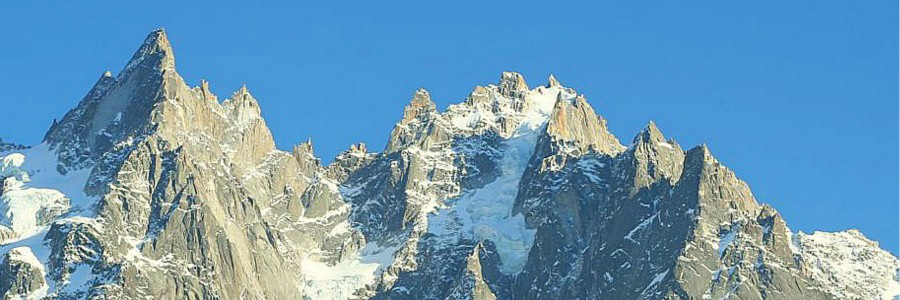
\includegraphics[width=0.5\textwidth]{./montblanc}
\caption{Mont Blanc.}
\label{fig:mont}
\end{center}
\end{figure}

\end{document}